\documentclass[11pt,oneside,a4paper,titlepage]{article}

\usepackage[most]{tcolorbox}

\usepackage{graphicx}
\usepackage{hyperref}
\hypersetup{
    colorlinks=true,
    linkcolor=blue,
    filecolor=magenta,
    urlcolor=blue
    }

\usepackage{geometry}
\geometry{
  a4paper,
  left=5mm,
  right=5mm,
  top=5mm,
  bottom=5mm
}

\definecolor{titleBack}{RGB}{0,66,21}

\title{Gabriel Tessier}
\date{}

\begin{document}
\tcbset{colframe=gray!95!black,colback=titleBack,arc=0mm}
\begin{tcolorbox}
  \begin{minipage}{4.5cm}
%    \hspace*{-0.3cm}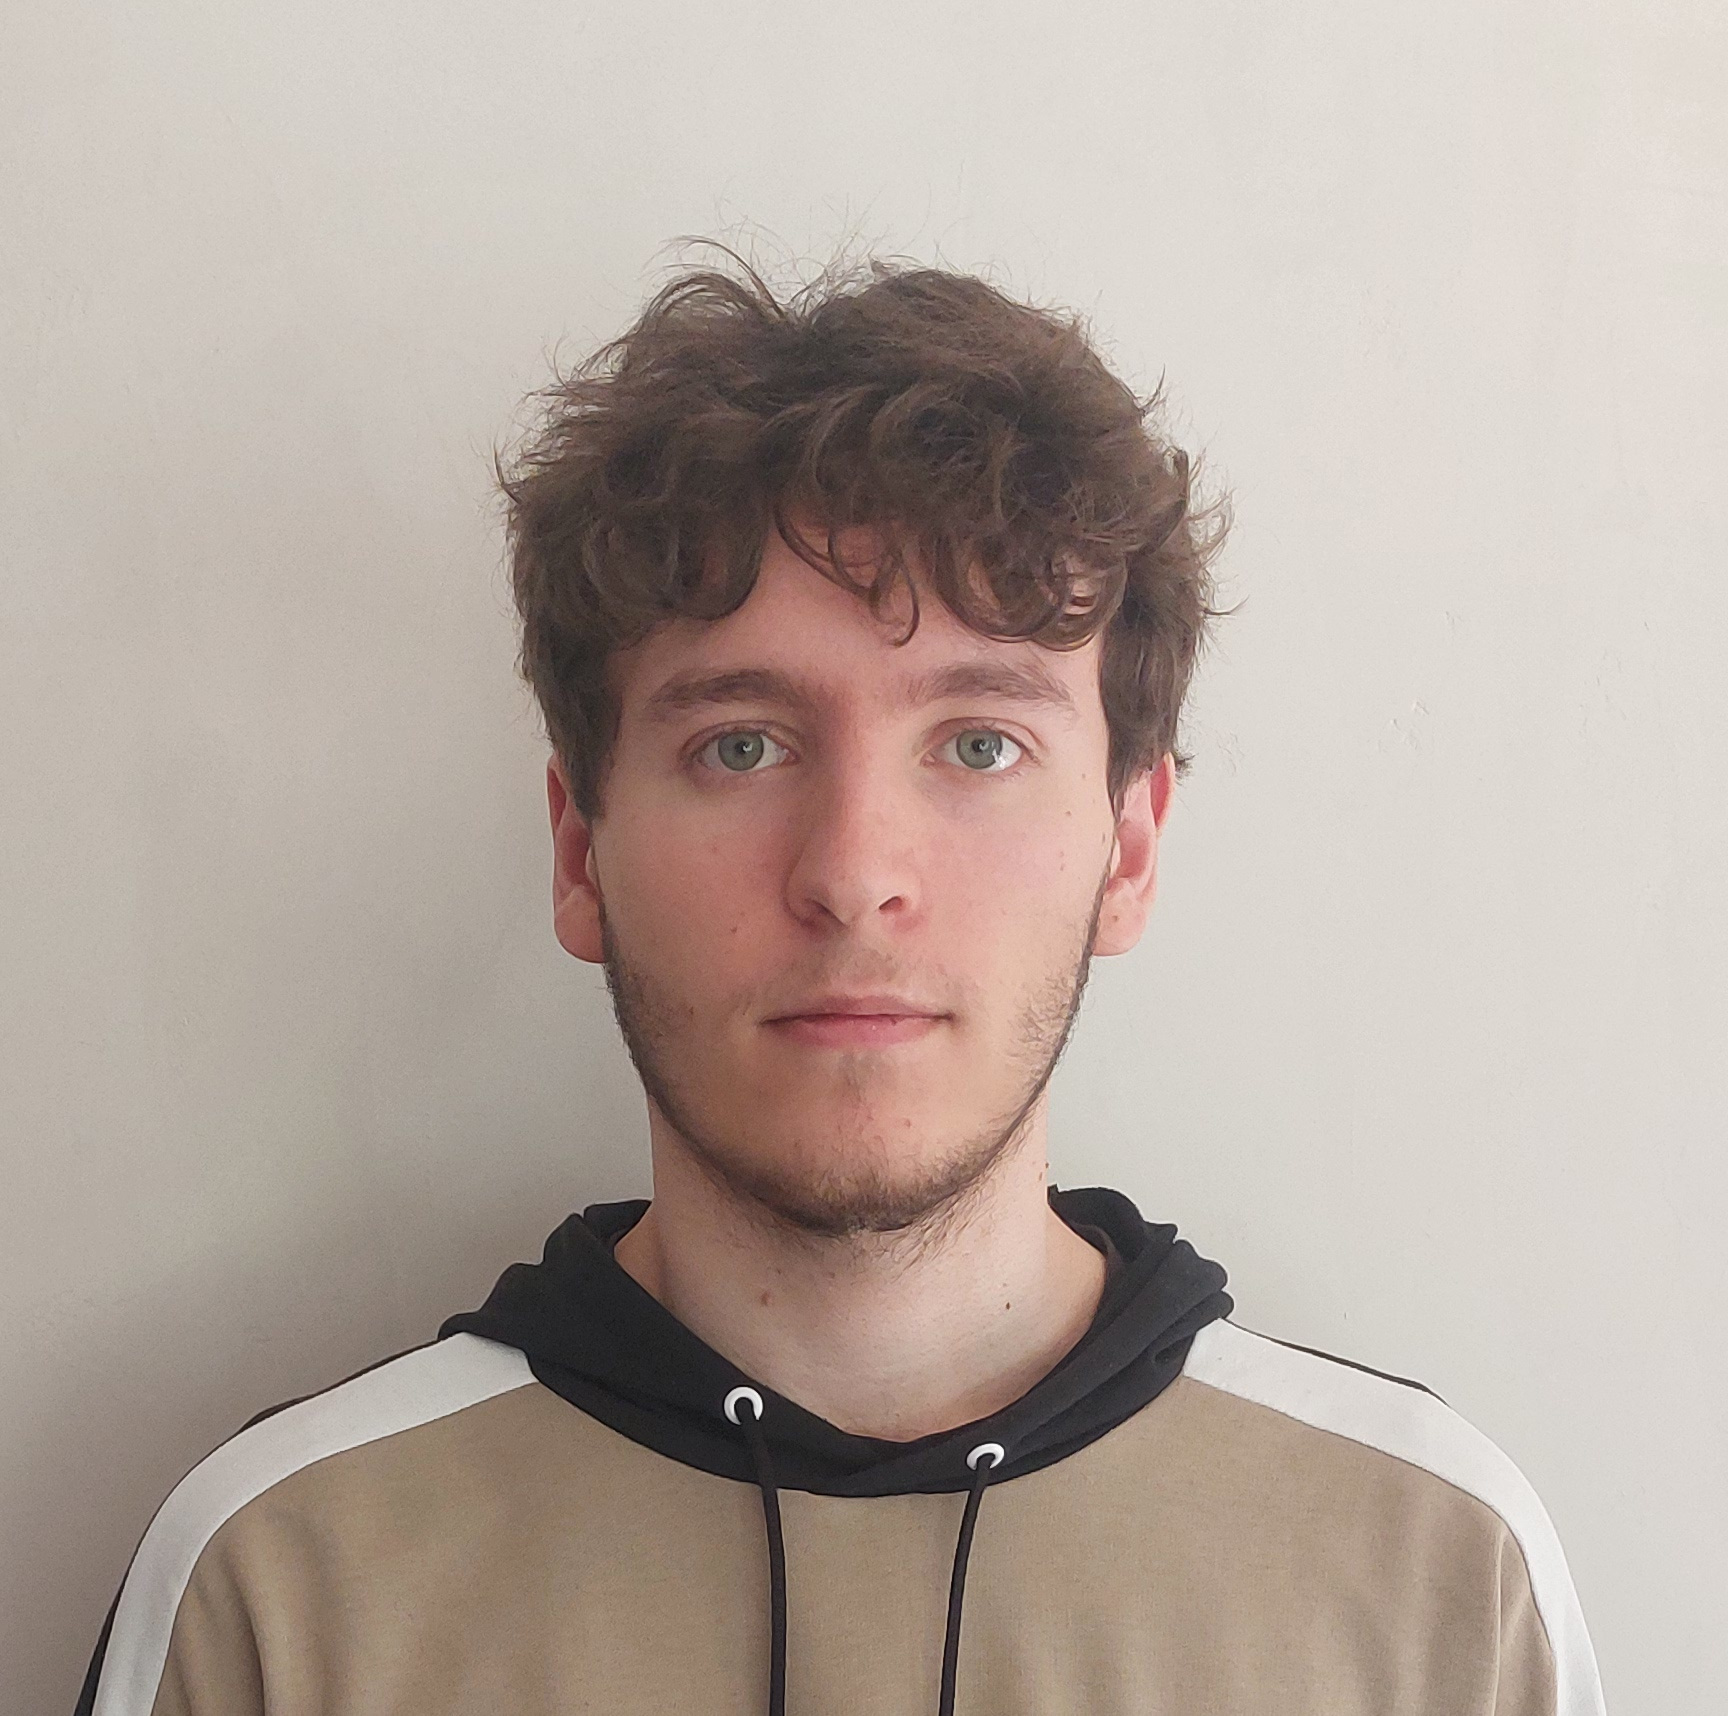
\includegraphics[width=4cm]{image.jpg}
    \begin{tikzpicture}
      \clip (0,0) circle (2cm) node {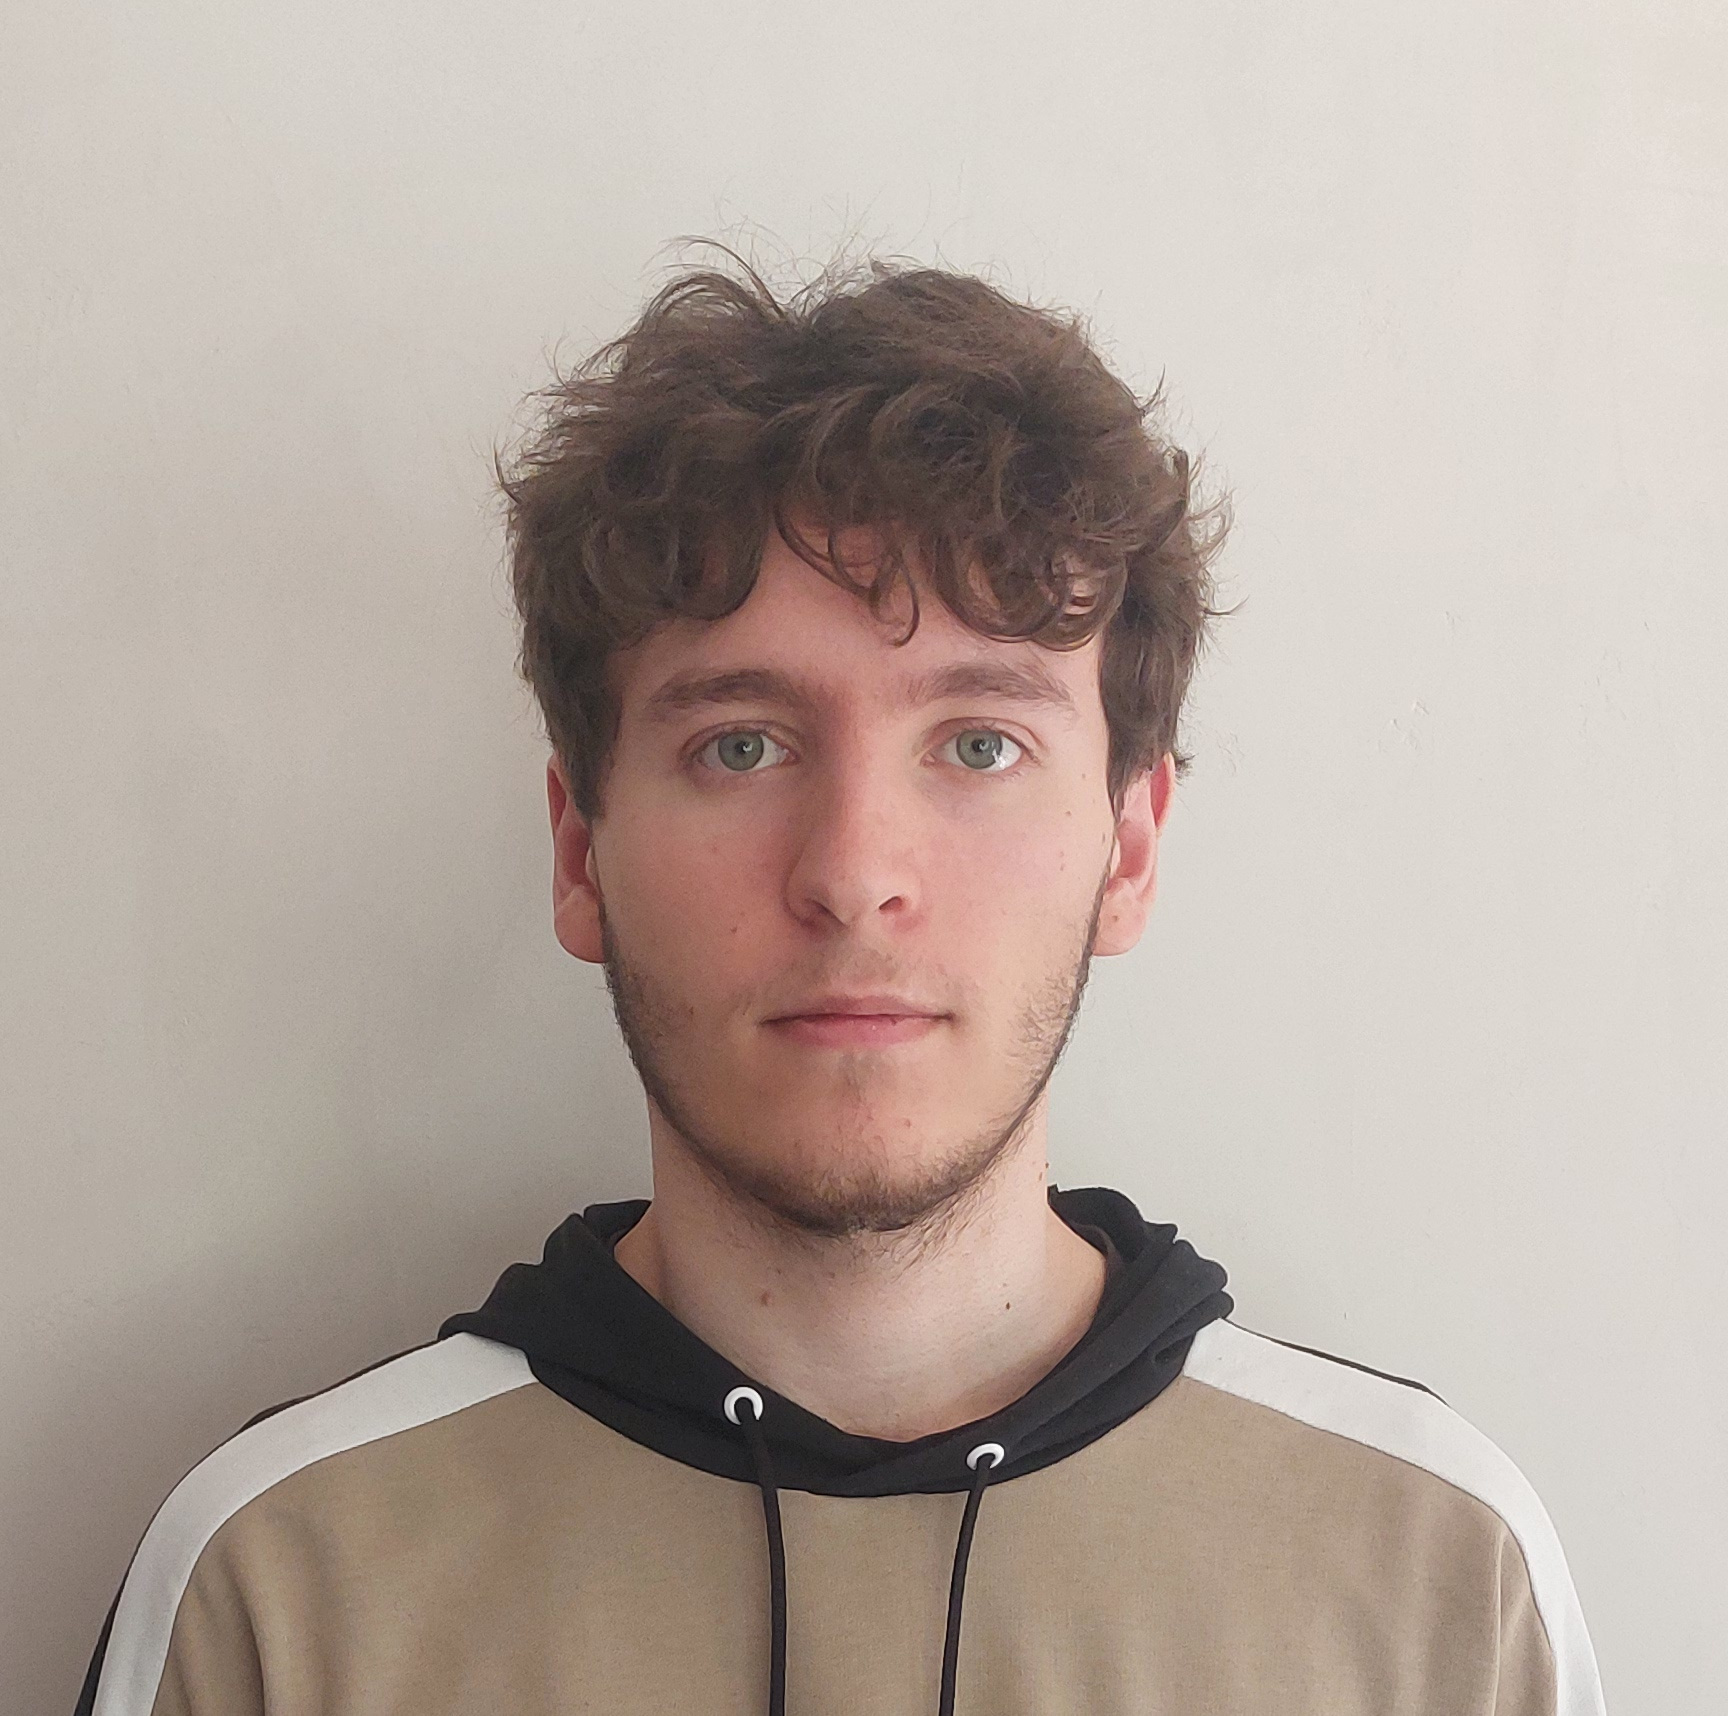
\includegraphics[width=4cm]{image.jpg}};
    \end{tikzpicture}
  \end{minipage}
  \begin{minipage}{15cm}
    \begin{center}
      \Huge{\textcolor{white}{Gabriel TESSIER}}\\
      \vspace*{0.5cm}
      \Large{\textcolor{white}{\emph{Étudiant Ensimag $2^{e}$ année}}}
    \end{center}
  \end{minipage}
\end{tcolorbox}

\tcbset{colframe=white,colback=white,arc=0mm}
\begin{tcolorbox}
  \begin{minipage}[t]{8cm}
    \vspace*{-0.5cm}
    \begin{tcolorbox}[grow to left by=0.6cm,colback=gray!25,colframe=white]
      \section*{Coordonnées}
      \setlength{\tabcolsep}{2pt}
      \begin{tabular}{rl}
        Tel : & 07 67 06 66 65 \\
        Email : & \href{mailto:Gabriel.Tessier45@gmail.com}{Gabriel.Tessier45@gmail.com} \\
        Github : & \href{https://github.com/GabrielTessier}{https://github.com/GabrielTessier} \\
        Permis : & B
      \end{tabular}

      \section*{Compétences}
      \begin{itemize}
        \item{Langages C / Assembleur x86\_64 et RISC-V / Ocaml / Java / Python / Kotlin / Lua}
        \item{Bases de données SQL}
        \item{OS Linux}
        \item{IDE Processing / Eclipse / Androïd Studio / Blender / VSCode / Emacs}
      \end{itemize}

      \section*{Langues}
      \begin{itemize}
        \item{Français}
        \item{Anglais}
      \end{itemize}

      \section*{Loisir}
      \begin{itemize}
        \item{Musique : pratique de la batterie pendant 10 ans en école de musique}
        \item{Informatique : programmation}
        \item{Lecture}
      \end{itemize}
    \end{tcolorbox}
  \end{minipage}
  \begin{minipage}[t]{11cm}
    \vspace*{-0.5cm}
    \begin{tcolorbox}[grow to right by=0.75cm,colframe=white,colback=white]
      \section*{Formation}
      \begin{itemize}
        \item{2025/2026 : $2^e$ année Ensimag}
        \item{2024/2025 : $1^{\text{er}}$ année Ensimag}
        \item{2023/2024 : CPGE MPI* au Lycée Descartes de Tours}
        \item{2022/2023 : CPGE MP2I au Lycée Descartes de Tours}
      \end{itemize}

      \section*{Diplôme}
      2021/2022 : Bac général, mention Bien
      \begin{itemize}
        \item{Spécialité Numérique et sciences informatiques (NSI)}
        \item{Spécialité Mathématiques}
        \item{Option Mathématiques expertes}
      \end{itemize}

      \section*{Stages}
      \begin{itemize}
        \item{Février 2020 : Stage de $2^{\text{de}}$ (1 semaine) à la Direction des Systèmes d'Information de l'Université d'Orléans.\\Découverte de la DSI : réseau, grande applications, système d'information (bases de données, connecteurs), développement web.}
        \item{Mars 2019 : Stage de $3^{\text{e}}$ (1 semaine) au LIFO (Laboratoire d'Informatique Fondamentale d'Orléans) - Université d'Orléans.\\Développement, pour un chercheur du laboratoire, d'une application pour télécommander un robot muni d'une carte Arduino avec un téléphone Androïd via Bluetooth.}
      \end{itemize}
    \end{tcolorbox}
  \end{minipage}
\end{tcolorbox}

\section*{Projets}
\subsection*{Création de joueurs artificiels pour Tetris}
Dans le cadre de mon TIPE en CPGE, j'ai programmé en langage C différentes stratégies de jeu pour Tetris (méthodes par apprentissage et avec heuristiques).
\subsection*{Décodeur jpeg vers ppm}
Dans le cadre d'un projet à l'Ensimag j'ai créer un décodeur jpeg en c.
\subsection*{Réalisation de plusieurs programmes}
Passionné par l'informatique depuis la classe de $5^{\text{e}}$, j'ai écrit de nombreux programmes avec différents langages de programmation (Java, Kotlin, Python, Ocaml, C, Lua, Javascript) et IDE (Processing, Eclipse, Androïd Studio).

\end{document}
